	In dem gestellten Problem geht es darum ein Netzwerkfluss von Eingang $o$ zu $n$ über die Knoten $a$ bis $d$ größtmöglich zu gestalten unter Beachtung verschiedener Bedingungen.Jeder Knoten hat nur Verbindungen zu bestimmten anderen Knoten bzw. Eingang un Ausgang $o$ und $n$. Diese Verbindungen können nur in eine Richtung benutzt werden und haben eine Höchstflussrate welche nicht überschritten werden darf. 
	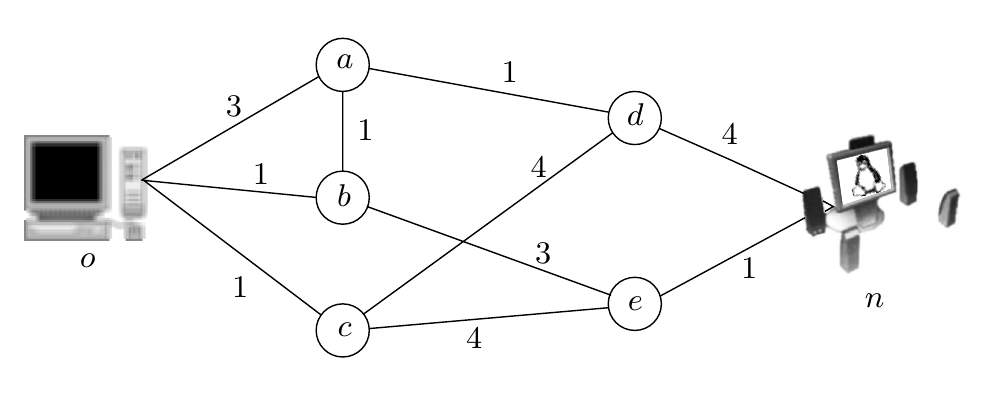
\includegraphics[width=\textwidth]{Grafiken/Netzwerkfluss_Bild.png}
	Also versuchen wir den Fluss zum letzten Knoten $o$ zu maximieren.
	\[ \max(f_{do}+f_{eo}) \]
	Um die maximale Kapazität der Verbindungen zu beachten werden folgende Ungleichungen eingeführt.Hierbei sind $i$ und $j$ zwei Knoten zwischen denen eine Verbindung besteht. $k_{ij}$ beschreibt die maximale Kapazität und $f_{ij}$ den tatsächlichen Fluss.Daraus ergibt sich für alle möglichen zulässigen $i$ und $j$:  
	\begin{align*}
		-k_{ij} \leq f_{ij} \leq k_{ij}
	\end{align*}
	Dabei gelten die Nebenbedingungen das der Fluss von einem Knoten genauso groß sein muss wie der Fluss von dem Knoten weg.Hierbei wird die Flussrichtung mit Vorzeichen berücksichtigt. Hierbei ist x ein beliebiger Knoten und j alle Knoten mit denen er verbindet.
	\begin{align*}
	0=\sum{f_{xj}}
	\end{align*}
	Wird dieses Lineare Programm gelöst so erhält man einen optimalen Fluss. 
	
	
	
	